\documentclass[aspectratio=169]{beamer}
\usepackage[no-math,deluxe,haranoaji]{luatexja-preset}
\renewcommand{\kanjifamilydefault}{\gtdefault}
\renewcommand{\emph}[1]{{\upshape\bfseries #1}}
\usetheme{metropolis}
\metroset{block=fill}
\setbeamertemplate{navigation symbols}{}
\usecolortheme[rgb={0.7,0.2,0.2}]{structure}
%%%%%%%%%%%%%%%%%%%%%%%%%%%
%% さまざまなアイコン
%%%%%%%%%%%%%%%%%%%%%%%%%%%
\usepackage{fontawesome}
%%%%%%%%%%%%%%%%%%%%%%%%%%%
\usepackage{tikz}
\usetikzlibrary{backgrounds}
\usepackage{tcolorbox}
\usepackage{xcolor}
\usepackage{amsmath}
%%%%%%%%%%%%%%%%%%%%%%%%%%%
%% 場合分け
\usepackage{cases}
%%%%%%%%%%%%%%%%%%%%%%%%%%%
% \myAnch{<名前>}{<色>}{<テキスト>}
% 指定のテキストを指定の色の四角枠で囲み, 指定の名前をもつTikZの
% ノードとして出力する. 図には remeber picture 属性を付けている
% ので外部から参照可能である.
\newcommand*{\myAnch}[3]{%
  \tikz[remember picture,baseline=(#1.base)]
    \node[draw,rectangle,#2] (#1) {\normalcolor #3};
}
%%%%%%%%%%%%%%%%%%%%%%%%%%%%
%% 音声リンク表示
\newcommand{\myaudio}[1]{\href{#1}{\faVolumeUp}}
%%%%%%%%%%%%%%%%%%%%%%%%%%%
% \myEmph コマンドの定義
%\newcommand{\myEmph}[3]{%
%    \textbf<#1>{\color<#1>{#2}{#3}}%
%}
\usepackage{xparse} % xparseパッケージの読み込み
\NewDocumentCommand{\myEmph}{O{} m m}{%
    \def\argOne{#1}%
    \ifx\argOne\empty
        \textbf{\color{#2}{#3}}% オプション引数が省略された場合
    \else
        \textbf<#1>{\color<#1>{#2}{#3}}% オプション引数が指定された場合
    \fi
}
%%%%%%%%%%%%%%%%%%%%%%%%%%%
\title{English is fun.\,\,{}---A Tale of Two cities---}
\author{}
\institute[]{}
\date[]

%%%%%%%%%%%%%%%%%%%%%%%%%%%%
%% TEXT
%%%%%%%%%%%%%%%%%%%%%%%%%%%%
\begin{document}
\begin{frame}[plain]
  \titlepage
\end{frame}

\section*{授業の流れ}
\begin{frame}[plain]
  \frametitle{授業の流れ}
  \tableofcontents
\end{frame}

\section{単数と複数}

\begin{frame}[plain]\frametitle{ひとつとふたつ以上}
\begin{columns}
\begin{column}{.2\textwidth}
\IfFileExists{./images/apple.png}{%
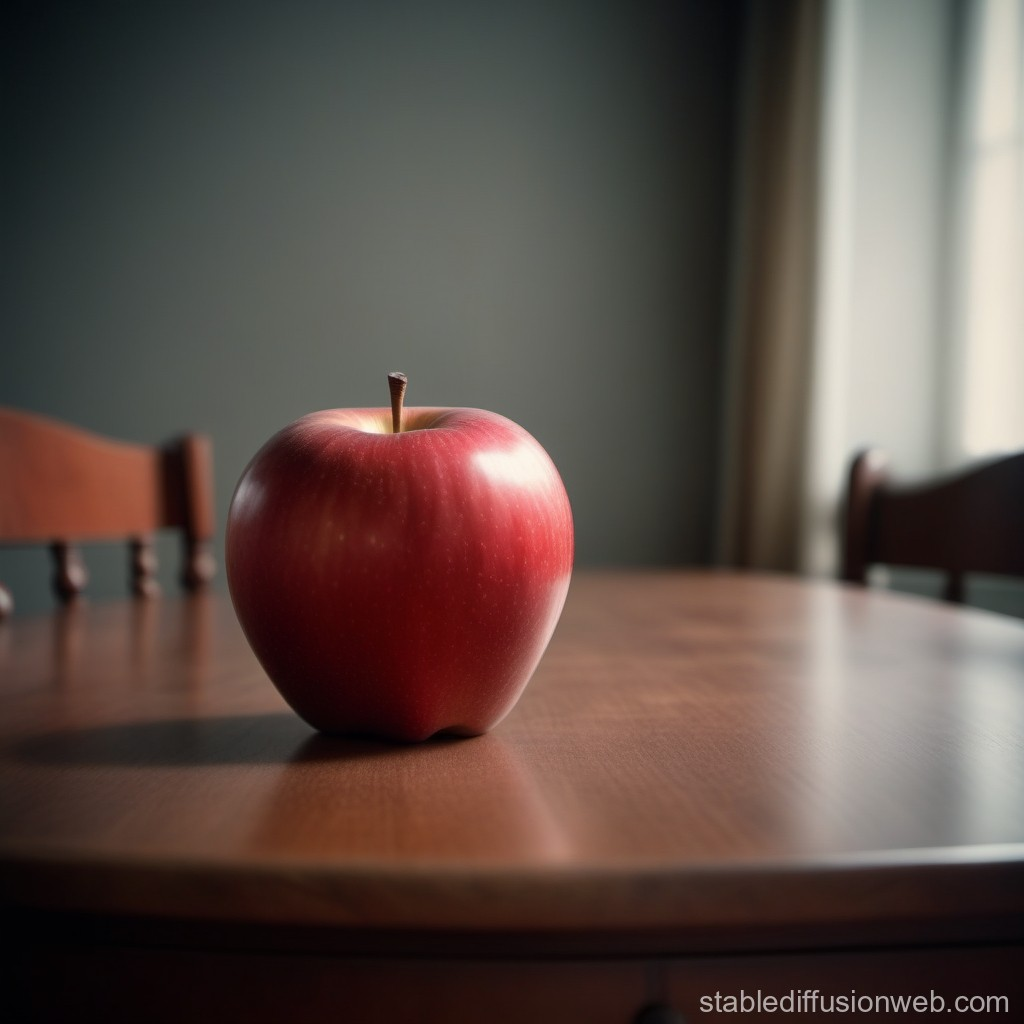
\includegraphics[width=.9\textwidth]{./images/apple.png}
}{naiyo}
\end{column}\pause
\begin{column}{.75\textwidth}\LARGE
a book
\end{column}
\end{columns}

\pause
\begin{columns}
\begin{column}{.2\textwidth}
\IfFileExists{./images/apple.png}{%
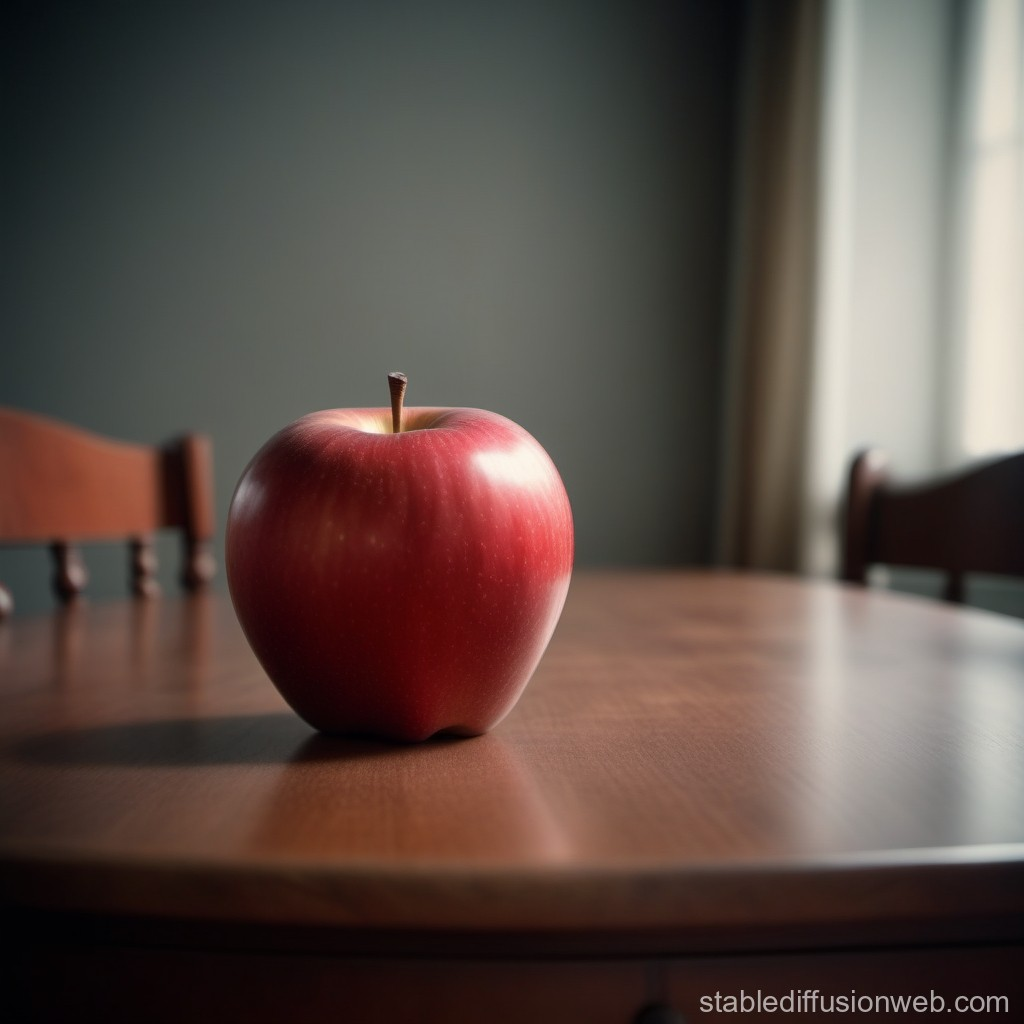
\includegraphics[width=.9\textwidth]{./images/apple.png}
}{naiyo}
\end{column}\pause
\begin{column}{.75\textwidth}\LARGE
two book\myEmph[4]{orange}{s}
\end{column}

\end{columns}
\end{frame}

\begin{frame}<1-10>[plain]\frametitle{日本語とのちがい}
\begin{columns}
\begin{column}[t]{.45\textwidth}
\begin{block}{日本語}
\onslide<2->{わたしは1冊の本を持っています。}

\onslide<3->{わたしは2冊の本を持っています。}

\onslide<4->{わたしは本を持っています。}
\end{block}
\end{column}
\begin{column}[t]{.45\textwidth}
\begin{block}{英語}
\onslide<5->{I have \textcolor{orange}{a book.}}

\onslide<6->{I have \textcolor{orange}{two books.}}

\onslide<7->*{I have \textcolor{red!50}{book}.}\onslide<8>{\,\,{}$\longleftarrow$これは\textcolor{red}{だめ}}
\end{block}
\end{column}
\end{columns}

\begin{exampleblock}<9->{Topics for Today}
\begin{itemize}
 \item<1->  \onslide<9,10>{\textcolor{orange}{単数形と複数形があります}}
 \item<2->  \onslide<10>{\textcolor{orange}{単数形を裸で使うことはできません}}
\end{itemize}
      \end{exampleblock}




\end{frame}


\begin{frame}<1-37>[plain,label=example]\frametitle{単数と複数}
 % \setbeamercovered{transparent}
  \begin{enumerate}
   \item<1-> \myEmph[14]{red}{I} \myEmph[15,27-29]{blue}{like} basketball. \onslide*<2>{わたしはバスケットボールが好きです。}\onslide*<31>{\footnotesize  like: 好き、好む basketball: バスケットボール}
   \item<3-> \myEmph[16]{red}{We} \myEmph[17,27-29]{blue}{walk} to school. \onslide*<4>{われわれは歩いて学校へ行きます。}\onslide*<32>{\footnotesize  walk: 歩く}
   \item<5-> \myEmph[18]{red}{They} \myEmph[19,27-29]{blue}{speak} English in Australia. \onslide*<6>{オースタラリアでは英語が話されています。}\onslide*<33>{\footnotesize  speak: 話す Australia:オーストラリア}
   \item<7-> \myEmph[20]{red}{I} \myEmph[21,27-29]{blue}{drink} tea every morning. \onslide*<8>{わたしは毎朝お茶を飲みます。}\onslide*<34>{\footnotesize  drink: 飲む tea: お茶 every morning: 毎朝}
   \item<9-> \myEmph[22]{red}{They} \myEmph[23,27-29]{blue}{study} math every day. \onslide*<10>{彼らは毎日数学を勉強します。}\onslide*<35>{\footnotesize study: 勉強する math: 数学 every day: 毎日}
   \item<11-> \myEmph[24]{red}{I} \myEmph[25,27-29]{blue}{play} the guitar. \onslide*<12>{わたしはギターをひきます。}\onslide*<36>{\footnotesize  play: (楽器などを)演奏する guitar: ギター}
  \end{enumerate}

\bigskip

\begin{exampleblock}<28->{Topics for Today}
\begin{itemize}
 \item<1->  \myEmph[28]{orange}{be動詞以外を一般動詞といいます}
 \item<2-> \myEmph[29]{orange}{一般動詞の意味はいろいろです}
\end{itemize}
      \end{exampleblock}


% Embed the sound file
\onslide<37>{%
\myaudio{./audio/004_verb_01.mp3}\,\,{}Listen carefully.(注意して聞いてください)
}



\end{frame}

\end{document}



